\documentclass{article}
\usepackage[utf8]{inputenc}
\title{Verification : Homework 8}
\author{Marius Belly - Le Guilloux}
\date{November 2021}


\usepackage{stmaryrd}   %N
\usepackage{esvect}     %Vector
\usepackage{hyperref}   %hypertext link
\usepackage{graphicx}
\usepackage{amsmath}    %overset
\usepackage{amssymb}    %square
\usepackage{amsthm}     %proof
\usepackage{xcolor}     %color
\usepackage{esvect}     %Vector
\usepackage{tikz}       %draw
\usetikzlibrary{positioning}
\usetikzlibrary{automata}
\usetikzlibrary{arrows}


%%% Operator %%%
\newcommand{\norm}[1]{\left\Vert #1 \right\Vert}
\newcommand{\card}[1]{\ensuremath{\left\|#1 \right\|}}
\newcommand{\interval}[2]{\ensuremath{\llbracket #1, \; #2 \rrbracket}}
\newcommand{\set}[1]{\{ #1 \}}
\newcommand{\br}[1]{\ensuremath{\llbracket #1 \rrbracket}} %Interpretation
\newcommand{\floor}[1]{\lfloor #1 \rfloor}
\newcommand{\ceil}[1]{\lceil #1 \rceil}
\newcommand{\ol}[1]{\overline{#1}}
\newcommand{\ul}[1]{\underline{#1}}

% Shortcuts sets
\newcommand{\bb}[1]{\mathbb{#1}}
\newcommand{\mc}[1]{\mathcal{#1}} %Abrev mathcal
\newcommand{\N}{\ensuremath{\mathbb{N}}}
\newcommand{\Z}{\ensuremath{\mathbb{Z}}}
\newcommand{\Q}{\ensuremath{\mathbb{Q}}}
\newcommand{\C}{\ensuremath{\mathbb{C}}}

%%% shorcuts logic %%%
\newcommand{\G}{\Gamma} % Abreviation pour logique etc..
\newcommand{\D}{\Delta} % Abreviation pour logique
\newcommand{\T}{\mathcal{T}} %Abreviation T pour logique

\newcommand{\V}{\mathcal{V}}
\newcommand{\A}{\mathcal{A}}
\newcommand{\R}{\mathcal{R}}


\begin{document}
\maketitle
\section*{Exercice 1}

\subsection*{a)}


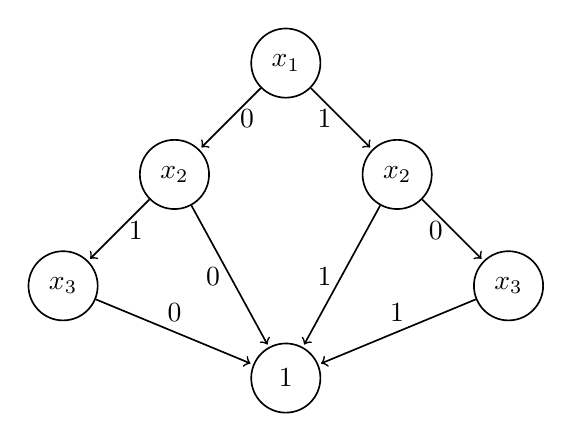
\begin{tikzpicture}[->,shorten >=1pt,auto,node distance=2cm,semithick]  
\node[state]   (A)                    {$x_1$};
\node[state]   (B) [below left of=A]  {$x_2$};
\node[state]   (C) [below right of=A] {$x_2$};
\node[state]   (D) [below left of=B]  {$x_3$};
\node[state]   (E) [below right of=C]  {$x_3$};
\node[state,draw=none]   (T) [below of=A]  {};
\node[state]   (F)   [below of=T]        {1};

\path (A)   edge [right] node {0} (B)
      (A)   edge [left] node {1} (C)
      (B)   edge [left] node {0} (F)
      (B)   edge [right] node {1} (D)
      (C)   edge [left] node {0} (E)
      (C)   edge [left] node {1} (F)
      (D)   edge [above] node {0} (F)
      (E)   edge [above] node {1} (F);

               
\end{tikzpicture}

\subsection*{b)}

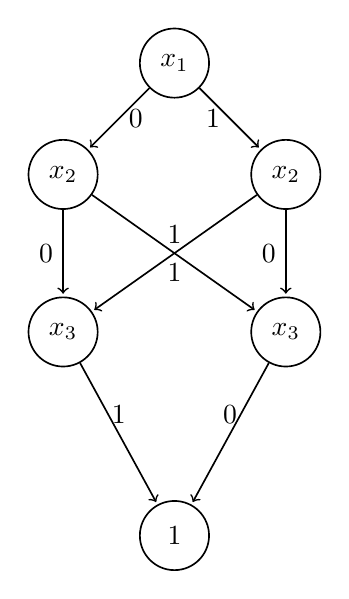
\begin{tikzpicture}[->,shorten >=1pt,auto,node distance=2cm,semithick]  
\node[state]   (A)                    {$x_1$};
\node[state]   (B) [below left of=A]  {$x_2$};
\node[state]   (C) [below right of=A] {$x_2$};
\node[state]   (D) [below of=B]  {$x_3$};
\node[state]   (E) [below of=C]  {$x_3$};
\node[state,draw=none]   (T1) [below of=A]  {};
\node[state,draw=none]   (T) [below of=T1]  {};
\node[state]   (F)   [below of=T]        {1};

\path (A)   edge [right] node {0} (B)
      (A)   edge [left] node {1} (C)
      (B)   edge [left] node {0} (D)
      (B)   edge [above] node {1} (E)
      (C)   edge [left] node {0} (E)
      (C)   edge [below] node {1} (D)
      (D)   edge [above] node {1} (F)
      (E)   edge [above] node {0} (F);

               
\end{tikzpicture}



\section*{Exercice 2}
\subsection*{a) $B(f)=1$}

Un tel BDD est de la forme
\newline
\begin{center}
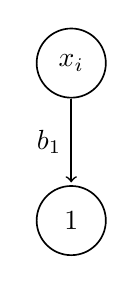
\begin{tikzpicture}[->,shorten >=1pt,auto,node distance=2cm,semithick]  
\node[state]   (A)                        {$x_i$};
\node[state]   (B) [below of=A]           {$1$};
\path (A)   edge [left] node {$b_1$} (B);
\end{tikzpicture}
\end{center}
\skip
Il y a $2n$ choix pour $x_i$ et $b_1$ donc $2n$ fonctions $f$ telle que $B(f)=1$



\subsection*{b) $B(f)=2$}


Un tel BDD est de la forme
\newline
\begin{center}
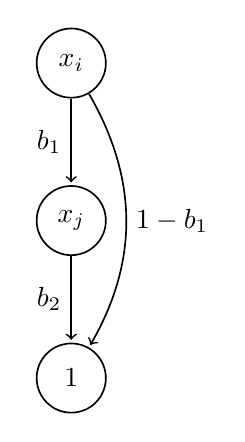
\begin{tikzpicture}[->,shorten >=1pt,auto,node distance=2cm,semithick]  
\node[state]   (A)                        {$x_i$};
\node[state]   (B) [below of=A]           {$x_j$};
\node[state]   (C) [below of=B]           {$1$};
\path (A)   edge [left] node {$b_1$} (B)
      (A)   edge [bend left,right] node {$1 - b_1$} (C)
      (B)   edge [left] node {$b_2$} (C);
\end{tikzpicture}
\end{center}
\skip
Il existe $\binom{n}{2}$ manières de choisir les étiquettes du BDD, 8 manières de choisir $b_1$ et $b_2$ et l'existence de l'arête étiquetée
Il y a donc en tout $4n(n-1)$ fonctions possibles.

\subsection*{c) $B(f)=3$} 

Les BDDs de taille 3 se divise en deux catégories : les arbres et les non arbres
$\bullet$ Comptons d'abord les premiers. Ceux-ci se divisent à nouveau en deux sous-catégories : les arbres de profondeur 2 et ceux de profondeur 3.\newline
$\bullet \bullet$ Les arbres de profondeur 2 sont de la forme 
\begin{center}
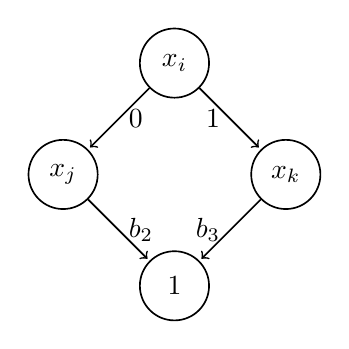
\begin{tikzpicture}[->,shorten >=1pt,auto,node distance=2cm,semithick]  
\node[state]   (A)                    {$x_i$};
\node[state]   (B) [below left of=A]  {$x_j$};
\node[state]   (C) [below right of=A] {$x_k$};
\node[state]   (D) [below right of=B] {$1$};
\path (A)   edge [right ] node {$0$} (B)
      (A)   edge [left] node {$1$} (C)
      (B)   edge [right] node {$b_2$} (D)
      (C)   edge [left] node {$b_3$} (D);
\end{tikzpicture}
\end{center}

Si $i,j$ et $k$ sont distinct alors il existe $2\binom{n}{3}$ manières de choisir puis répartir les étiquettes du BDD et 4 manières de choisir $b_1$ et $b_2$.\newline
Sinon, $j=k$. Il existe alors $\binom{n}{2}$ manières de choisir les étiquettes du BDD et $b_1 = 1-b_2$, d'où deux manières de choisir $b_1$ et $b_2$.\newline
Finalement, il existe $8\binom{n}{3} + n(n-1)$ fonctions dont le BDD est un arbre de taille 3 et de profondeur 2.\newline
$\bullet \bullet$ Les arbres de profondeur 3 sont de la forme 
\begin{center}
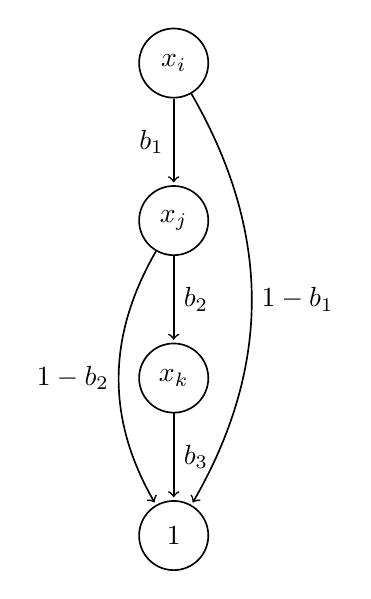
\begin{tikzpicture}[->,shorten >=1pt,auto,node distance=2cm,semithick]  
\node[state]   (A)               {$x_i$};
\node[state]   (B) [below of=A]  {$x_j$};
\node[state]   (C) [below of=B] {$x_k$};
\node[state]   (D) [below of=C] {$1$};
\path (A)   edge [left] node {$b_1$} (B)
      (A)   edge [bend left,right] node {$1-b_1$} (D)
      (B)   edge [right] node {$b_2$} (C)
      (B)   edge [bend right,left] node {$1-b_2$} (D)
      (C)   edge [right] node {$b_3$} (D);
\end{tikzpicture}
\end{center}

$i,j$ et $k$ sont nécessairement distincts donc il existe $\binom{n}{3}$ manières de choisir les étiquettes du BDD, 8 manières de choisir $b_1,b_2$ et $b_3$ et 4 manière de choisir l'existence des arètes étiquetées $1-b_1$ et $1-b_2$.\newline
Il y a donc en tout $32\binom{n}{3}$ fonctions dont le BDD est un arbre de taille 3 et de profondeur 2.\newline
$\bullet$ Comptons maintenant les BDD qui ne sont pas des arbres, c'est à dire les BDD de la forme
\begin{center}
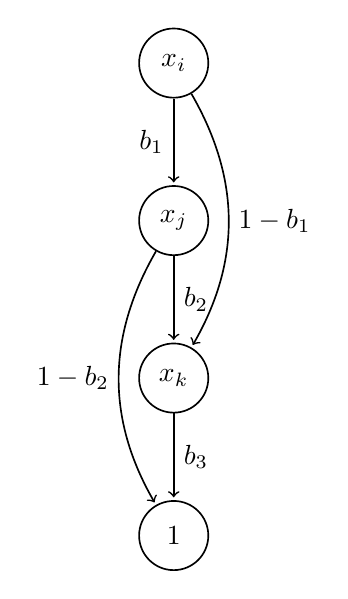
\begin{tikzpicture}[->,shorten >=1pt,auto,node distance=2cm,semithick]  
\node[state]   (A)               {$x_i$};
\node[state]   (B) [below of=A]  {$x_j$};
\node[state]   (C) [below of=B] {$x_k$};
\node[state]   (D) [below of=C] {$1$};
\path (A)   edge [left] node {$b_1$} (B)
      (A)   edge [bend left,right] node {$1-b_1$} (C)
      (B)   edge [right] node {$b_2$} (C)
      (B)   edge [bend right,left] node {$1-b_2$} (D)
      (C)   edge [right] node {$b_3$} (D);
\end{tikzpicture}
\end{center}
$i,j$ et $k$ sont nécessairement distincts donc il existe $\binom{n}{3}$ manières de choisir les étiquettes du BDD, 8 manières de choisir $b_1,b_2$ et $b_3$ et 2 manière de choisir l'existence de l'arête étiquetée $1-b_2$.\newline    
Il y a donc en tout $16\binom{n}{3}$ fonctions dont le BDD est de taille 3 mais n'est pas un arbre.
\newline
\newline
Finalement, il existe $n(n-1) + 56\binom{n}{3}$ fonctions $f$ telle que $B(f)=3$





\newpage


\end{center}
%0b2_+1(1-b2)_ -> 3*2=6
%0b2_+1_b3 ->  2*4=8
%(1-b1)__+b1(1-b2)_+b1b2b3 -> 8*4=32
%(1-b1)_b3 + b1b2b3


\end{document}


